\documentclass[a4paper]{article}
\usepackage[margin=1.25in]{geometry}
\usepackage{amsmath}
\usepackage{ragged2e}
\usepackage[table,xcdraw]{xcolor}
\title{Radioactivity - The Absorption of Gamma Rays by Matter}
\date{February 8, 2018}
\author{Pablo Sevilla}
\usepackage{graphicx} 
\usepackage{float}
\usepackage{subcaption}

\begin{document}
  \pagenumbering{gobble}
  \maketitle
  \newpage
  \pagenumbering{arabic}
  
  \section*{Abstract}
  This experiment was conducted with the ultimate goal of measuring the absorption coefficient $\mu$ of lead under mono-energetic gamma ray radiation. Preliminary experiments were done to calculate the intrinsic properties of a SPECTECH ST369 Radiation Counter, measure backgroud radiation, verifying the validity of Poisson Distributions and measuring the dead time of pulses caused by gamma rays in a Geiger-Muller Tube. We found that count rate followed the Poisson Distribution model with a confidence of 66.4 per cent. We also found that the absorption coefficient for a gamma ray of $0.662MeV$ is $1.0457\frac{1}{cm}$.
  
  \section{Introduction}
  \subsection{Cesium-137}
  This experiment granted us with the opportunity to study gamma-ray radiation. The chosen radioactive sample is Cesium-137, a well known isotope that emits mono-energetic gamma rays and $\beta$ particles. It has a half life of about 30 years. Thanks to this property, radioactive intensity could be accurately treated as a constant across the duration of the experiment. The decay scheme of Cesium-137 is the following:
  
  \begin{figure}[h]
  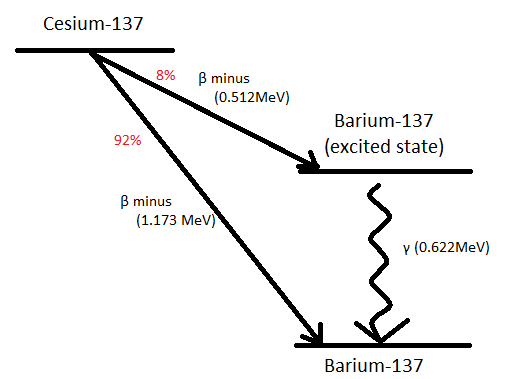
\includegraphics[scale=0.75]{Cs-137.png} 
  \centering
  \caption{Cesium-137 Decomposition Layout}
  \end{figure}
  
As we are only interested in the gamma decay, beta particles needed to be blocked in order to not incorrectly measure them as gamma rays. This was achieved thanks to the clever geometry of the sample. The active cesium is placed inside a plastic cylinder in such a way that it is closer to one end than the other. As gamma rays are unaffected by plastic but $\beta$ particles are not, the manufactured sample outputs both particles via one end, and only gamma-rays through the opposite end.
  
  Radioactive materials decay at random times. The probability of decaying in a time interval $\Delta t$ is $p=\beta \Delta t$, where $\beta$ is a constant of proportionality. Assuming we start with a large number of particles, we can approximate the number of decayed particles as $\Delta N=pN$. Equating both equations and integrating over infinitesimal time intervals $dt$, we obtain:
  \begin{equation} 
  \label{nuclei} 
  N(t)=N_0e^{-\beta t}
  \end{equation}
  where $N_0$ is the number of particles at time $t=0$ and $1/\beta$ is the mean lifetime of a nucleus (43.3 years).
  As we are interested in the decay rate of the sample, we can differentiate with respect to time to obtain the following relationship:
  \begin{equation} 
  \label{decayrate} 
  \frac{d}{dt}N(t)=\beta N_0e^{-\beta t}=\beta N(t)
  \end{equation}
  As previously mentioned, under a time considerably shorter than the mean lifetime $1/\beta$, the decay rate can be approximated as constant.
  
  Due to the random nature of radioactivity, the count rate is often modeled with a Poisson Distribution. Hence the probability of detecting $m$ particles is:
  \begin{equation} 
  \label{decayrate} 
  P(m)=e^{-\lambda}\frac{\lambda^{m}}{m!}
  \end{equation}
where $\lambda$ is the mean number of counts. 

Such model's validity will be tested during a preliminary experiment.
  \subsection{Gamma Ray Detection}
  As a gamma ray detector, we have used the notorious device developed by Hans Geiger and Walther Muller in 1908, the Geiger-Muller tube. Such device uses a cylindrical container with an inert gas in it, Argon. Inside it, we can find a wire going through the middle from side to side of the cylinder. An external potential difference is applied between this wire (anode) and the internal sides of the container (cathode). 
 
  \begin{figure}[h]
  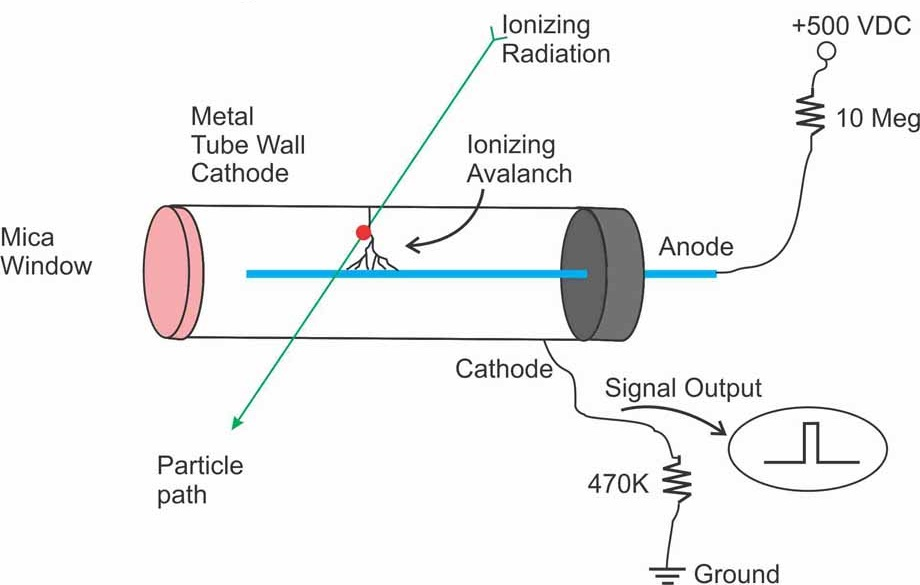
\includegraphics[scale=0.8]{geiger-muller.jpg} 
  \centering
  \caption{Geiger-Muller Tube}
  \end{figure}
  
  If gamma rays bombard the device, there is a possibility that they will give out their energy to an electron in an Argon atom, giving it enough energy to escape the nucleus electrostatic attraction. The new energetic free electron will be attracted to the anode, and as the electron is attracted quite abruptly, ionizing shocks will occur due to energetic collisions. This will over saturate the surroundings of the anode with positively charged ions. Such saturation will induce a relatively strong signal, serving as the output of the G-M tube. This signal will decay and therefore it will be treated as a pulse across the duration of this investigation.
  
  \subsection{Apparatus}
  In order to study the pulses of the Geiger-Muller Tube, other devices need to be used to count and quantify these outputted voltage pulses. The chosen devices were a SPECHTECH counter and an oscilloscope:  
  
  \begin{figure}[h]
  \centering
  \begin{subfigure}[h]{0.4\linewidth}
  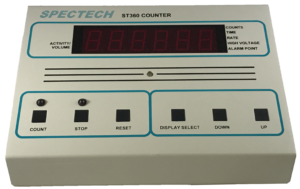
\includegraphics[width=\linewidth]{Counter.png}
  \end{subfigure}
  \begin{subfigure}[h]{0.4\linewidth}
  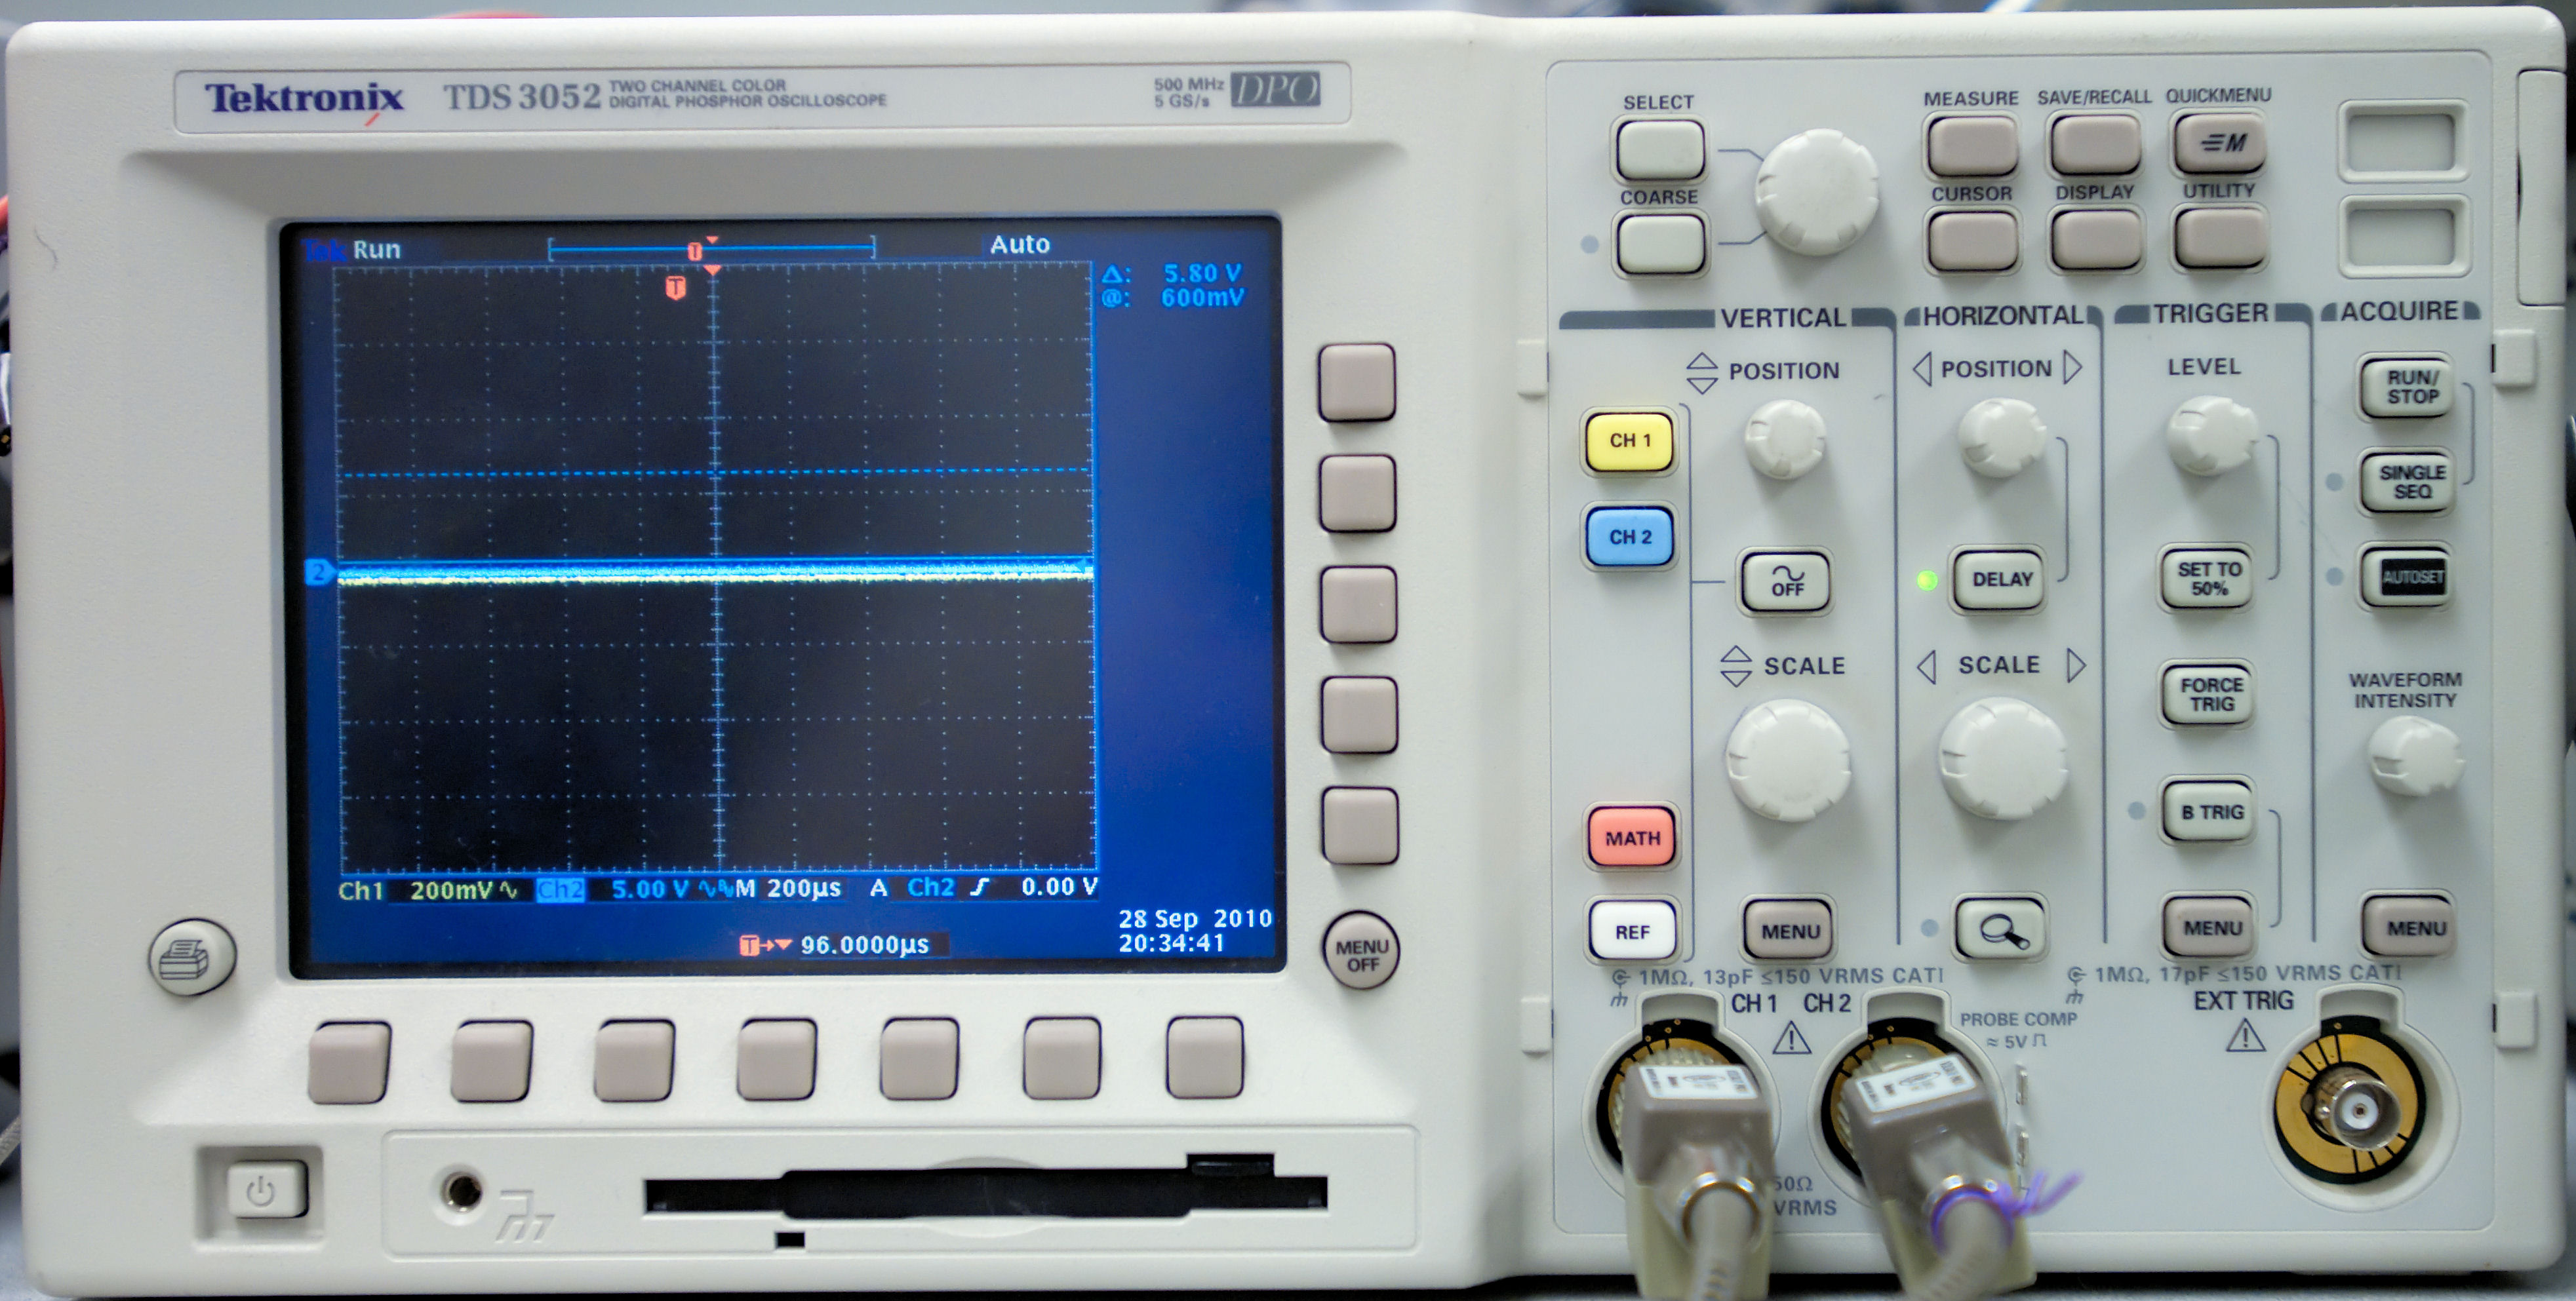
\includegraphics[width=\linewidth]{oscilloscope.jpg}]
  \end{subfigure}
  \caption{\textbf{Left:}  A SPECTECH ST360 Radiation Counter was used to     count pulses 
  \textbf{Right:} A Tektronix TDS 3052 Oscilloscope was used to measure pulse properties, such as amplitude and decay time.}
  \end{figure}
  Due to the limitations of the counter, only pulses greater than a specific threshold between $-0.4V$ and $-1.0V$ can be recorded by the device. As the counter also has a voltage supply option, a reasonably high voltage will be used in order for the electrons to have enough kinetic energy to create avalanches. Supply voltages higher than $900V$ will not be used to avoid a continuous discharge of the G-M tube, which would make it unable to detect radiation.
  
  \section{Procedure}
  \subsection{Preliminary Experiments}
  \subsubsection{Pulse Shape and Intrinsic Properties}
  The following schematic circuit for counting and investigating pulses will be used: 
  \begin{figure}[h]
  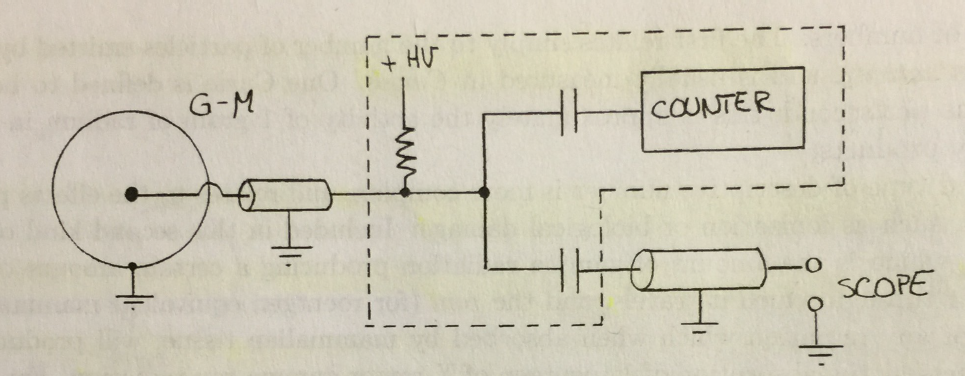
\includegraphics[scale=0.8]{circuitdiagram} 
  \centering
  \caption{The dashed line represents our counter device. It contains a charging resitor and two capacitors that cut off its high supplied voltage. They do not affect the lower voltage pulse information that is passed on to the oscilloscope.}
  \end{figure}
  
  The Cesium-137 source was placed under the G-M Tube, under its gamma ray only configuration ($\beta$ particles would ionize Argon too). When a pulse is produced by the G-M Tube, its signal is recorded by the counter and passed on to the oscilloscope to measure its magnitude and decay time.
  
  As previously mentioned, the limitations of the counter arise the problem of a threshold supply voltage. Low voltages will not give enough kinetic energy to the electrons to induce ionizing shocks. These ionizing collisions are very useful because they then create electron avalanches, allowing for a strong, detectable signal. On the other hand, single electrons would hardly induce a potential difference. It is only once this threshold is surpassed that we will be able to obtain signals. It is important to notice the existence of an upper limit to the supply voltage. A very strong voltage will create a continuous discharge that will disable the G-M tube. In order to find such threshold, count rate data was taken for a range of supply voltages.
  
  The decay of the pulse was another substantial factor needed to be tweaked for increased accuracy in detecting gamma rays. The time constant follows the relationship $\tau=RC$, while the amplitude goes like $A=Q/C$, where $Q$ is the charge collected by the anode. When connecting an extrinsic known capacitor $C_k$ or a known resistor $R_k$, time constants and amplitudes will change as follows:
  
 \centering
  \begin{tabular}{lr}
$C_k$ & $R_k$\\
\hline
$\begin{aligned}[t]
\tau=R(C+C_k)\\
A=Q/(C+C_k)
\end{aligned}$ & $\begin{aligned}[t]
\tau=[(RR_k)/(R+R_k)]C_k\\
A=Q/C
\end{aligned}$ 
\end{tabular}
\justify

  Furthermore, the time constants were measured using the oscilloscope's cursor function alongside with the following useful property: Exponentially decaying pulses decay to $\frac{1}{2}$ of its peak value at a time $T_{1/2}$ equal to $ln (2)$ times the time constant. Using the relationships above, the observed intrinsic properties were reported.
  
  During the discharge of the pulse, the G-M Tube is unable to record another pulse until the pulse has essentially disappeared. This is what is referred as 'dead time'. This results in possible ionizing agents not being detected, decreasing the accuracy of our experiment. Due to this nature, we are mostly interested in shortening the decay time. A shorter decay translates to a brief "dead-time", and hence a greater accuracy. From looking at the equations in the table above, we can conclude that an extrinsic resistor would shorten the duration of the pulse. For this reason, an extrinsic resistor with a value of $9.96 k\Omega$ was used.
  
  \subsubsection{Counts due to Background Radiation}
  In order to increase the accuracy of the experiment, background radiation needed to be considered. For that, the supply voltage was set to a voltage higher than the previously calculated threshold of $720V$. The chosen voltage was $840V$, and this supply voltage remained constant in all further measurements. With this idea in mind, the source was placed far away from the detector so the G-M tube only detects background radiation from sources such as cosmic rays.
  
  The timer function of the counter was used to measure background counts over three periods of time of 1000 seconds. The average was taken and divided by 1000 to obtain the background radiation in counts/second.
  \subsubsection{Counting Statistics}
  The source was placed at a distance so that 5 to 10 counts per second were detected. The counts were recorded for 100 one second intervals, while the frequency of each detected emission was recorded.
This frequency distribution was compared to the model of a Poisson distribution. In order to asses the fitness of such model, a Chi Squared analysis was performed
on the data by:
\begin{equation} 
  \label{chisquared} 
\chi^{2}=\sum_{i=1}^{v} \frac{(x_i-\mu_i)^{2}}{\sigma_i^{2}}
  \end{equation} 
 
  where  $x$ is the count rate value, $\mu$ is the mean and $\sigma$ is the standard deviation.The $\chi^{2}$ goodness of fit tells us how confident we can be when stating that such distribution can be modeled with Poisson Statistics.
\subsubsection{Measuring the Counter Dead Time}
  We previously introduced the concept of dead time. It is important to quantify this property for greater understanding of the results. The quantity was estimated by using the $\beta$ particle configuration, therefore obtaining an much greater amount of pulses per unit time. Setting the oscilloscope in Persistence Mode (where every new pulse is superimposed on the old pulses), we achieved something analogous to the following:
  
  \begin{figure}[h]
  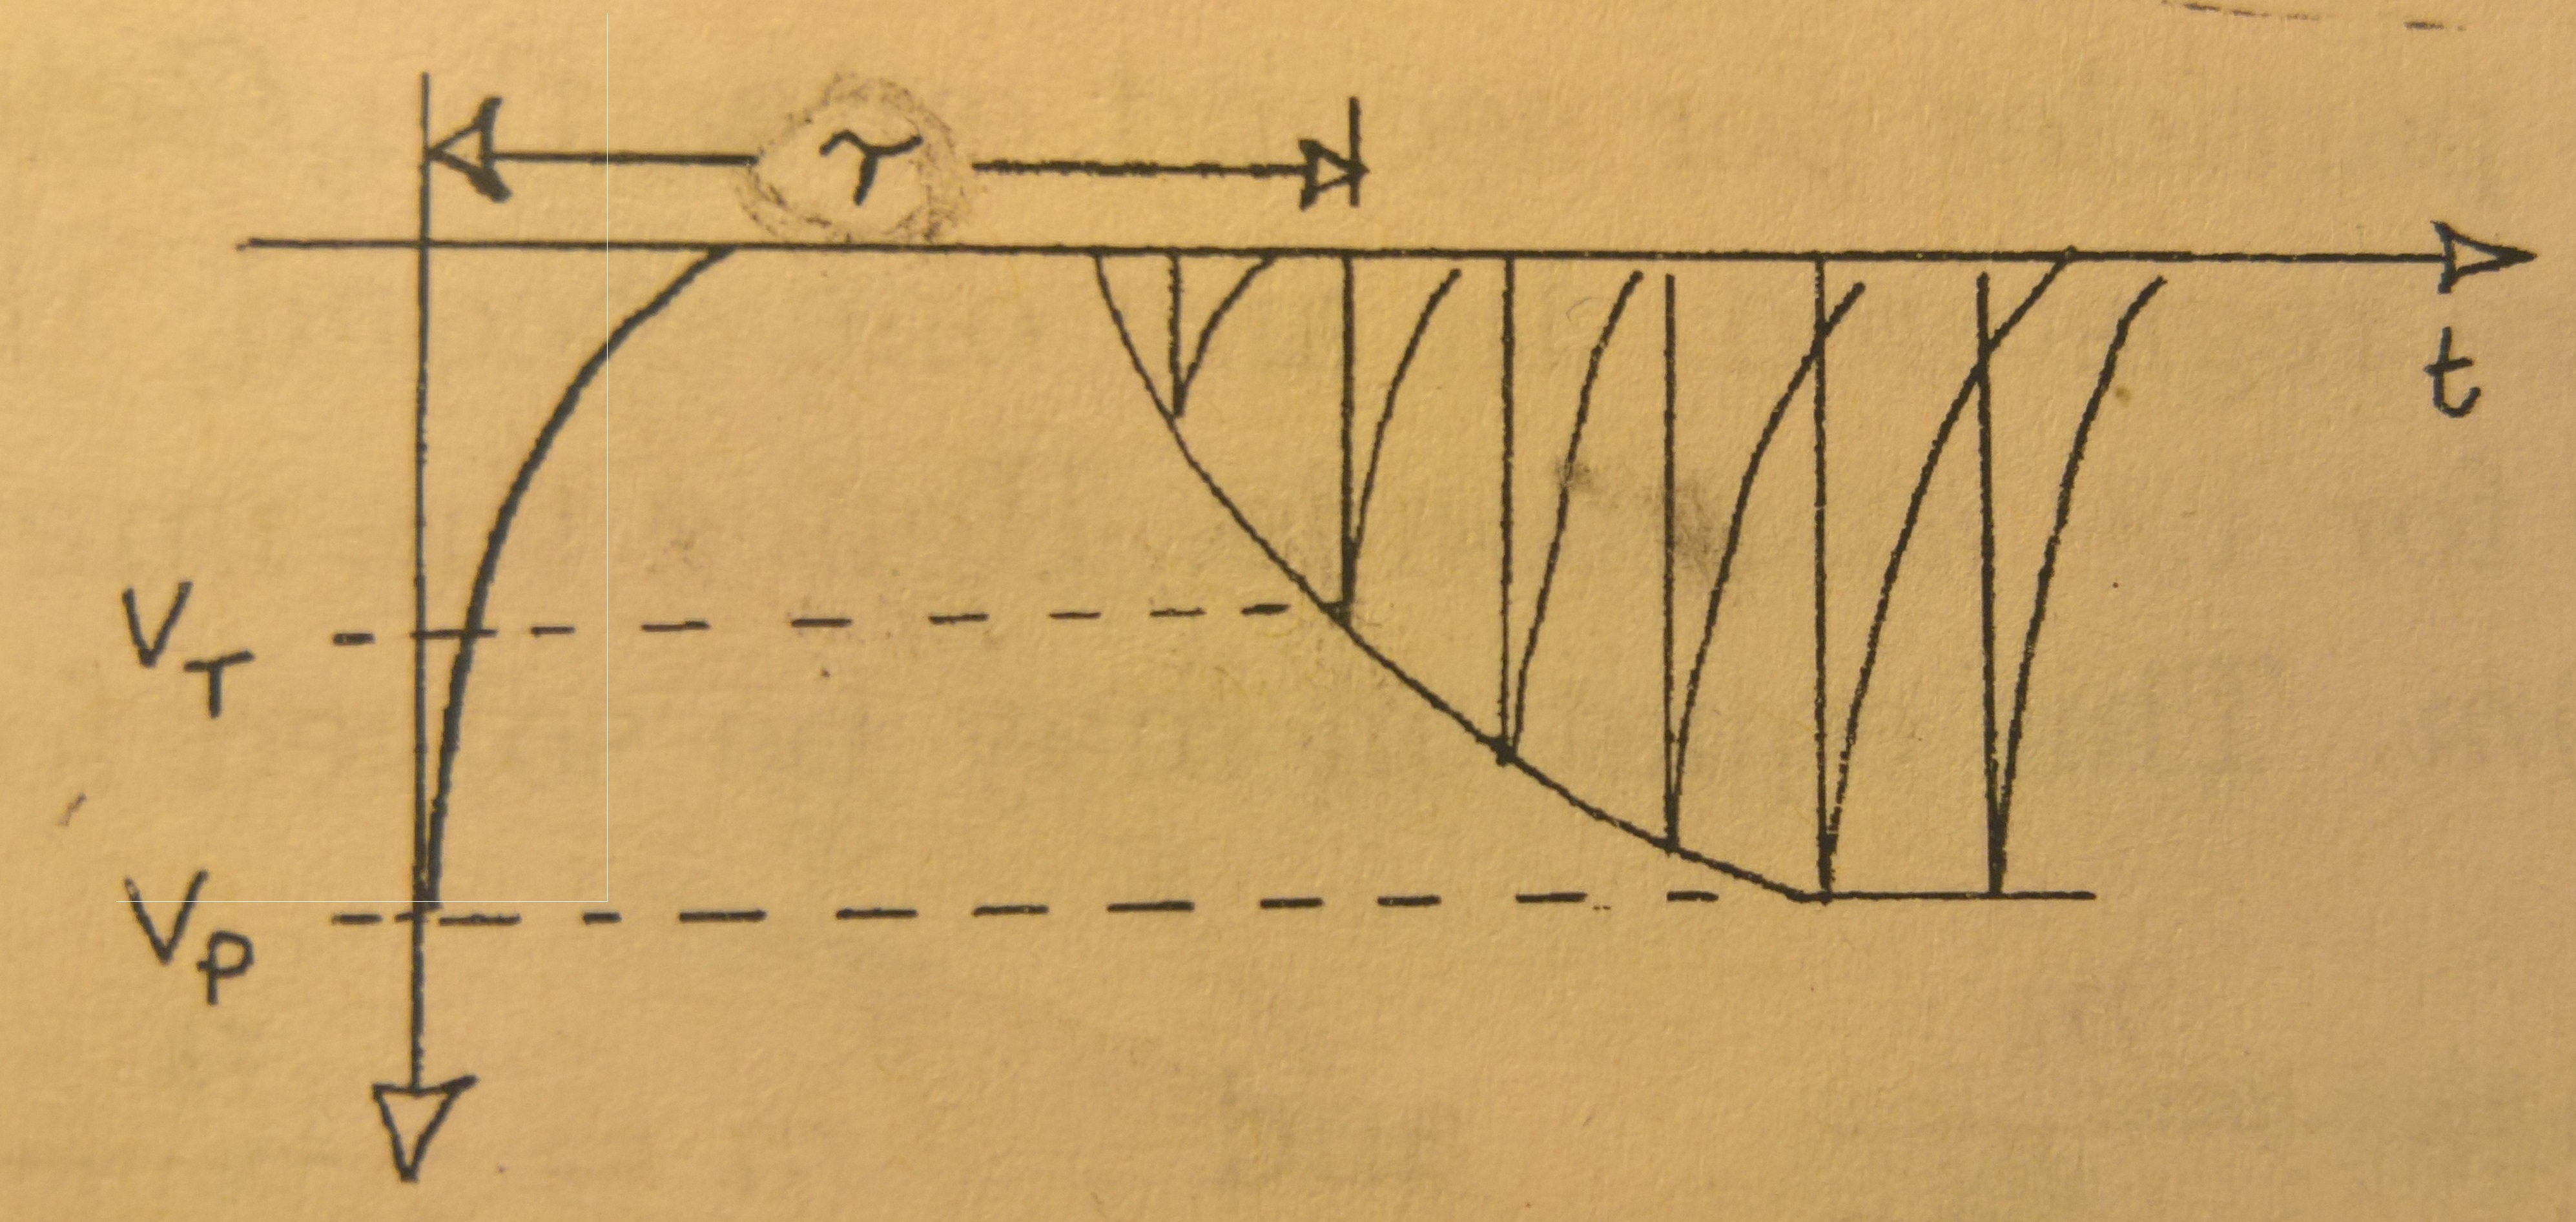
\includegraphics[scale=0.05]{deadtime} 
  \centering
  \caption{$V_p$ corresponds to the pulse amplitude, while $V_T$ is the trigger threshold. It is not until this threshold is surpassed that pulses are again countable.}
  \end{figure}
  
  Using such configuration, alongside with the cursor function of the oscilloscope, the dead time $\tau$ was calculated.
  
  \subsection{Absorption of Gamma Rays by Lead}
  Once all preliminary experiments were finished and our apparatus was correctly set up and tweaked, we were ready to move on to the heart of the experiment; measuring the absorption coefficient $\mu$ of lead. In order to do so, count rate was measured under varying thicknesses of lead. Lead thickness was calculated by measuring the weight of the lead blocks and dividing it by the cross-sectional area. This method is much more efficient than manually measuring the thickness, as there is a lot of room for human error for the latter. Rulers often are not precise enough to tell small differences between two thin plates. Also, the metal plates are not perfectly uniform so a direct measurement of its thickness might be too inaccurate. Once we had a set of 5 lead blocks, different combinations were used to obtain 7 datapoints of intensity vs thickness.
  
  The absorption coefficient $\mu$ can be found using the following relationship:
  \begin{equation}
  I=I_{0}e^{-\mu x}
  \end{equation}
  
  where $I_0$ is the original intensity with no lead, and $x$ is the thickness of the combined lead blocks between the source and the G-M Tube. Background radiation will be needed to be considered in this part of the experiment by subtracting it from the raw data. If we take the natural logarithm of both sides of Equation (5), we obtain the following:
  
  \begin{equation}
  ln(I)=ln(I_0)-\mu x
  \end{equation}
  
  This equation is particularly useful as plotting a graph of $ln(I)$ versus $x$ results in a straight line of gradient $-\mu$ and $y$-intercept of $ln(I_0)$.
  
 \section{Data and Analysis}
 \subsection{Preliminary Experiments}
 \subsubsection{Pulse Shape and Intrinsic Properties}
 The task at hand was to investigate the count rate as a function of supply voltage. We know that a threshold voltage exist where electron gain sufficient kinetic energy to create ionizing shocks and therefore avalanches. Also, a maximum voltage exists where the gas is continuously discharged and avalanches can no longer occur. We need to plot a graph of count rate for a different number of supply voltages. The results obtained are the following:
 
 \begin{figure}[h]
  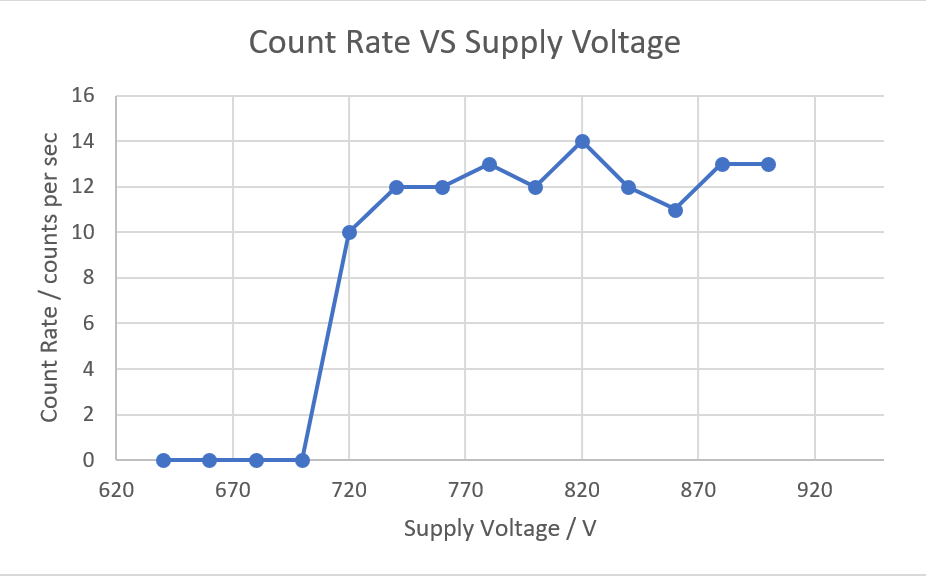
\includegraphics[scale=0.75]{plateau} 
  \centering
  \caption{We found the threshold voltage to be $720V$}
  \end{figure}
  
  From the picture above, we see that the lowest supply voltage with a non-zero count rate is $720V$, and therefore this is the threshold. The behavior after the threshold seems kind of arbitrary. From the reading of the lab manual and online resources, we would expect to find a region where the count rate reaches a plateau, or in other words a constant count rate. Unfortunately, the graph obtained is not exactly flat anywhere, varying from 11-14 count rates for higher supply voltages than the threshold. This behavior was probably caused by the random nature of radioactivity; it is spontaneous and the only way to tell if it's going to decay in a time $\delta t$ is with a probability and not a certainty. For future reference, a counter measure for this would be replicating this preliminary experiment many more times, so that an average can be taken and this random nature would be less predominant in the graph.
 
In addition, we also needed to find the values for the the intrinsic charge, capacitance and resistance of our setup. We found these using the previously mentioned  relationships between amplitude, extrinsic and intrinsic capacitance/resistance, charge and time constant $\tau$. Using some algebra, we found these values to be the following:

\begin{table}[h]
\centering
\label{my-label}
\begin{tabular}{lllll}
\cline{1-4}
\rowcolor[HTML]{C0C0C0} 
\multicolumn{1}{|l|}{\cellcolor[HTML]{C0C0C0}}              & \multicolumn{1}{l|}{\cellcolor[HTML]{C0C0C0}Charge (nC)} & \multicolumn{1}{l|}{\cellcolor[HTML]{C0C0C0}Intrinsic Capacitance (nF)} & \multicolumn{1}{l|}{\cellcolor[HTML]{C0C0C0}Intrinsic Resistance ($\Omega$)} &  \\ \cline{1-4}
\multicolumn{1}{|l|}{\cellcolor[HTML]{EFEFEF}Average Value} & \multicolumn{1}{c|}{7.7}                                 & \multicolumn{1}{c|}{7.7}                                                & \multicolumn{1}{c|}{850}                                                     &  \\ \cline{1-4}
                                                            &                                                          &                                                                         &                                                                              &  \\
                                                            &                                                          &                                                                         &                                                                              & 
\end{tabular}
\end{table}

These obtained values make sense with the nature of the setup. The intrinsic capacitance needs to be rather small in order to block the high voltage to the oscilloscope while still sending the information about the signal pulse made by the G-M tube. The capacitance value, $7.7nF$ is indeed very small compared to the extrinsic capacitor that we used. 

\subsubsection{Counts due to Background Radiation}
The average background radiation was found to be 0.45 counts per second. Such calculation was made using the setup without the Cesium-137 source, but it was placed relatively far away. As we know that the radiation follows the inverse square law, a separation of a couple of meters was enough to treat the experiment as 'background radiation only'. The setup was turned on and left to count for 100 seconds. This was repeated two more times and then an average of the three experiments was taken. An improvement to this experiment would have been taking data inside a lead box so radiation from the background was minimized. This rather subtle modification would have surely improved both the accuracy and the precision of the experiment.

\clearpage

\subsubsection{Counting Statistics}
In this preliminary experiment, we wanted to verify the validity of the Poisson Distribution Model in relation to our data. With that in mind, a sample of 100 count rates was obtained and plotted in a graph. From this sample we calculated its mean and variance. A Poisson Distribution with the same mean was calculated and superimposed with our previously obtained graph. In addition, the chi-squared test was made to quantitatively assess the fitness of this model to our data. Our obtained results are the following:

\begin{figure}[h]
  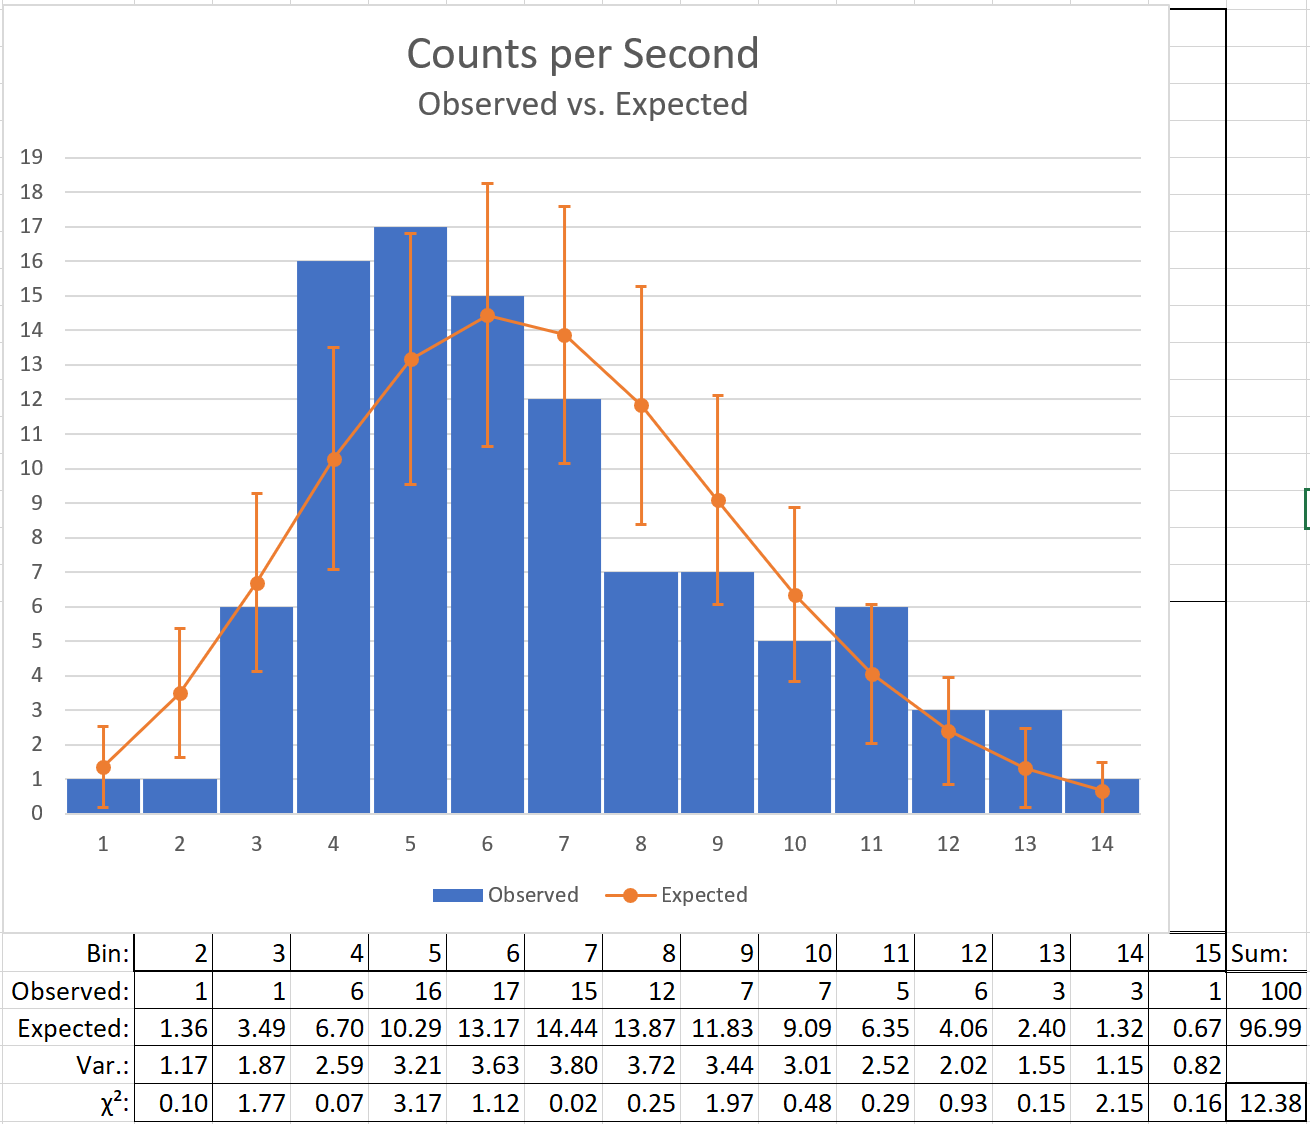
\includegraphics[scale=0.75]{countingstatistics2} 
  \centering
  \caption{Distribution of Count Rates for 100 measurements. Using the $\chi^{2}$ goodness of fit, expected values were calculated for each bin.}
  \end{figure}
  
  As we can see from the graph, our data is somewhat consistent with the Poisson Model. The orange line represents a Poisson Distribution with the same mean as our data. Also, we have computed error bars for the Poisson Model by the use of the following relation:
    
  \begin{equation}
  s_n = \sqrt{\frac{\mu}{n}}
  \end{equation}
  
  where $\mu$ is the mean value and $n$ is the bin number. As some of the bins do not lie within the Poisson Distribution error bars, the chi square goodness of fit will be lower than 100 per cent. It seems that the data is skewed to the left, where lower bin numbers seem to have more occurrences. This might be due to some limitation in our apparatus (such as the intrinsic dead time), or even simply due to the random nature of radioactivity. 
  
  The following data corresponds to the chi-squared goodness of fit, as described in the lab manual. The computed confidence level is the following:
  
  
  \begin{figure}[h]
  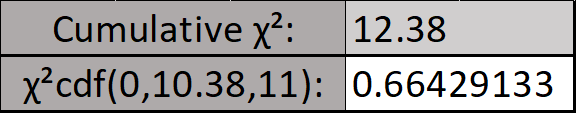
\includegraphics[scale=1.0]{chisquared} 
  \centering
  \caption{The $\chi^{2}$ goodness of fit with our given mean gave us this one-sided confidence level. The confidence turned out to be $66.4$ per cent.}
  \end{figure}

Some might argue that the confidence level obtained is not high enough (see Figure 8). This is caused by the skew to the left on Figure 7. Again, a bigger data sample might be done in the future to perhaps obtain a better fit.

  \subsubsection{Measuring the Counter Dead Time}
  A very important factor to this experiment is the dead time. This is the amount of time after a pulse that the G-M tube is unable to detect another pulse. It was important to minimize this dead time as much as possible to minimize the probability of missing an avalanche ultimately caused by a gamma ray. The duration of this dead time is strongly related to the accuracy of detecting the gamma rays. As previously mentioned, the use of an extrinsic resistor helped us shorten this dead time, and therefore a relatively strong extrinsic resistor of $9.96k\Omega$ was used in the setup. Using the PERSISTENCE MODE on the oscilloscope, we were able to superimpose new pulses against old pulses and, using the voltage trigger threshold, calculate the dead time. The results found for our setup are the following:
  
  \begin{figure}[h]
  \centering
  \begin{subfigure}[h]{0.4\linewidth}
  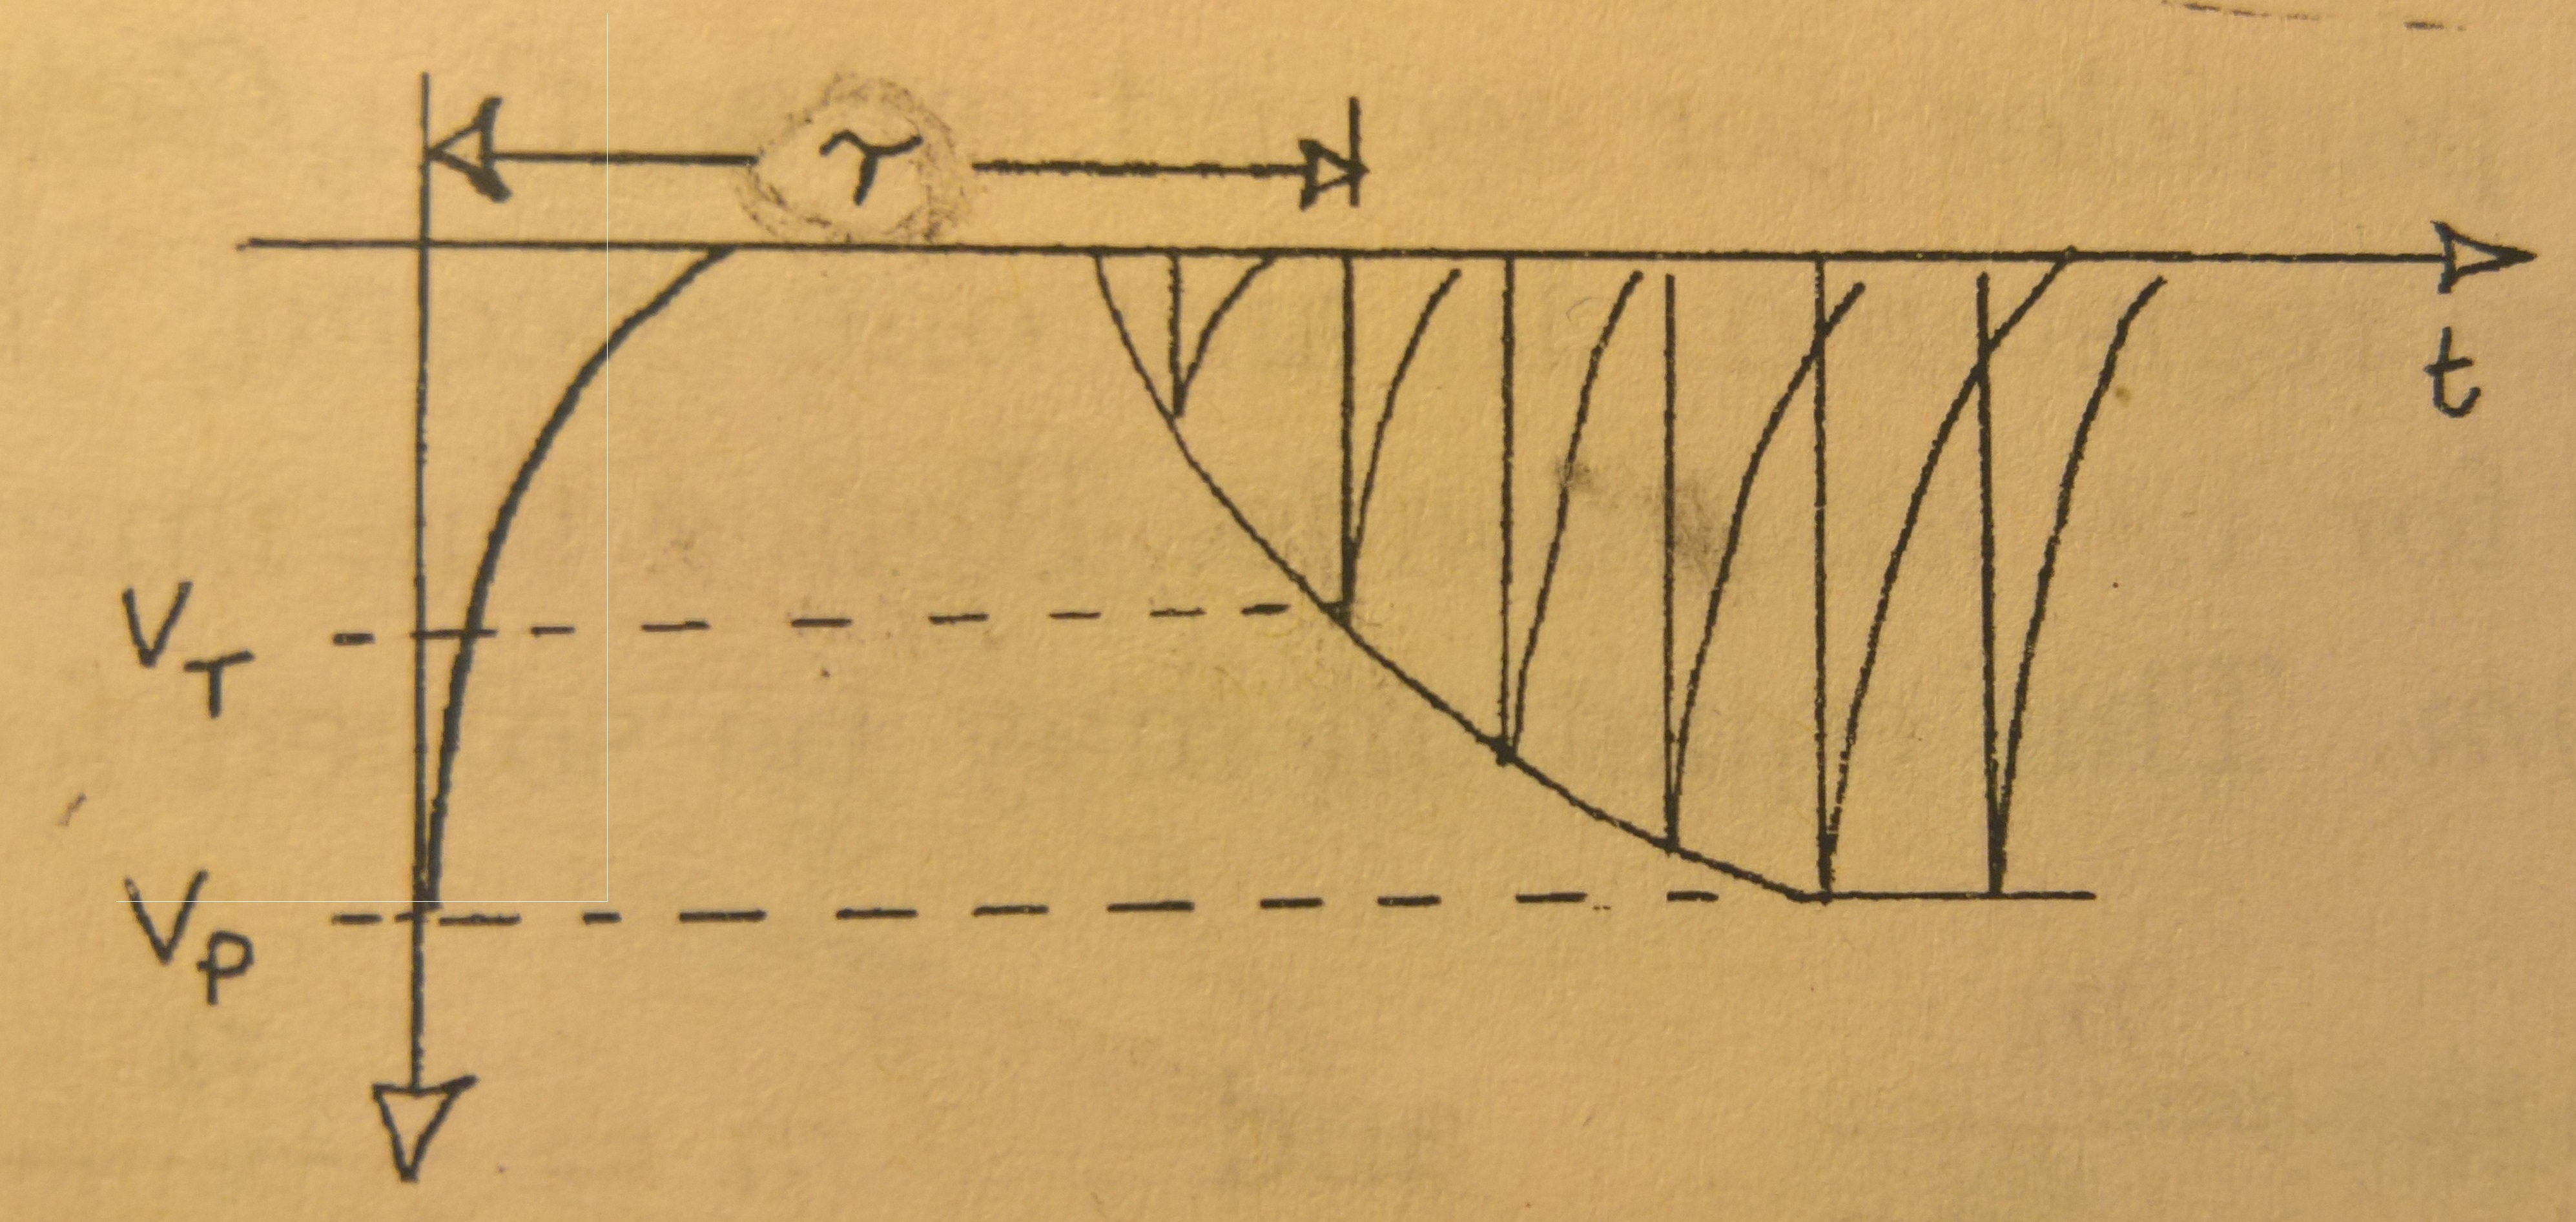
\includegraphics[width=\linewidth]{deadtime}
  \end{subfigure}
  \begin{subfigure}[h]{0.4\linewidth}
  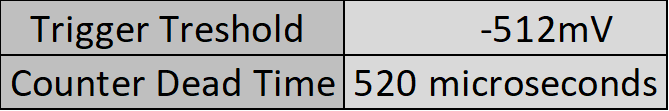
\includegraphics[width=\linewidth]{measureddeadtime}]
  \end{subfigure}
  \end{figure}
  
  The measured counter dead time is consistent with the range discussed in the lab manual. There it was stated that dead time is usually a few hundred micro seconds. This is what we got by looking at the oscilloscope, 
 
 \subsection{Absorption of Gamma Rays by Lead}
 Gamma rays are blocked by lead, a rather dense material. However, if the thickness of the lead shielding is not large enough, some gamma rays might be lucky enough to pass the material without being absorbed or deflected. In order to calculate quantitatively how much lead blocks gamma rays, several different lead plates were used. The lead plates, labeled from A to E, have the following mass, surface area and thickness:
  
 \begin{figure}[h]
  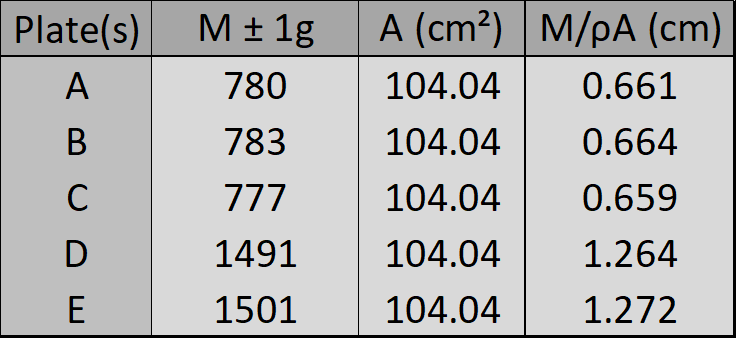
\includegraphics[scale=1.5]{plates} 
  \centering
  \end{figure}
  
  For future experiments, it might be useful to account for errors in both the surface area and the mass of the plates. We took them as definite values for simplicity. The mass uncertainty was neglected as it counted for a very small percentage error of the actual value. However, the surface area was also neglected, but the percentage error was much bigger due to the lack of precision of the ruler used. This is a flaw of the experiment and should definitely be corrected in a future experiment.
  
  Several combinations of lead blocks were used to obtain a data sample of 7 data points of gamma ray intensity $I$ vs thickness $x$. The intensity is analogous to the count rate given by the G-M tube. To this intensity, or counts per second, the background radiation was subtracted from all distinct data points. This increased our accuracy in the experiment. Using the following relationship;
  
    \begin{equation}
  I=I_{0}e^{-\mu x}
  \end{equation}
  
  where $\mu$ is the absorption coefficient. A plot of intensity (or counts per second) versus lead thickness ($x$) was made. This are the results found:
  
   \begin{figure}[h]
   \centering
  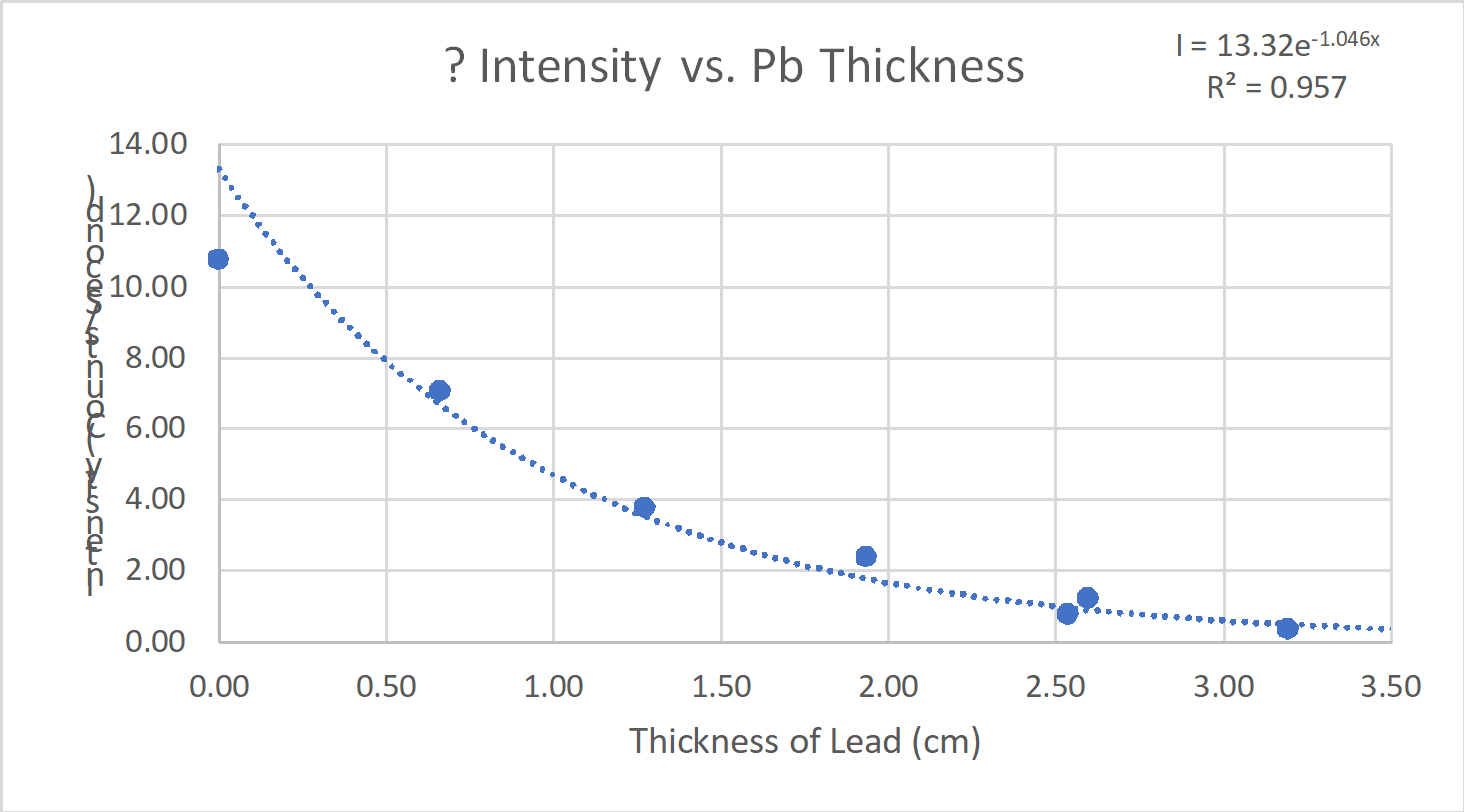
\includegraphics[scale=0.5]{ivsx} 
  \end{figure}
  
  In order to extract the absorption coefficient out of this data, it is useful to take the logarithm of equation $(7)$, where we obtain the following linear relationship between $ln(I)$ and lead thickness $x$:
  
    \begin{equation}
  ln(I)=ln(I_0)-\mu x
  \end{equation}
  
  Plotting this new equation, we can see that we will obtain a straight line with a negative slope. The magnitude of this slope will be equal to the absorption coefficient $\mu$. 
  
   \begin{figure}[h]
  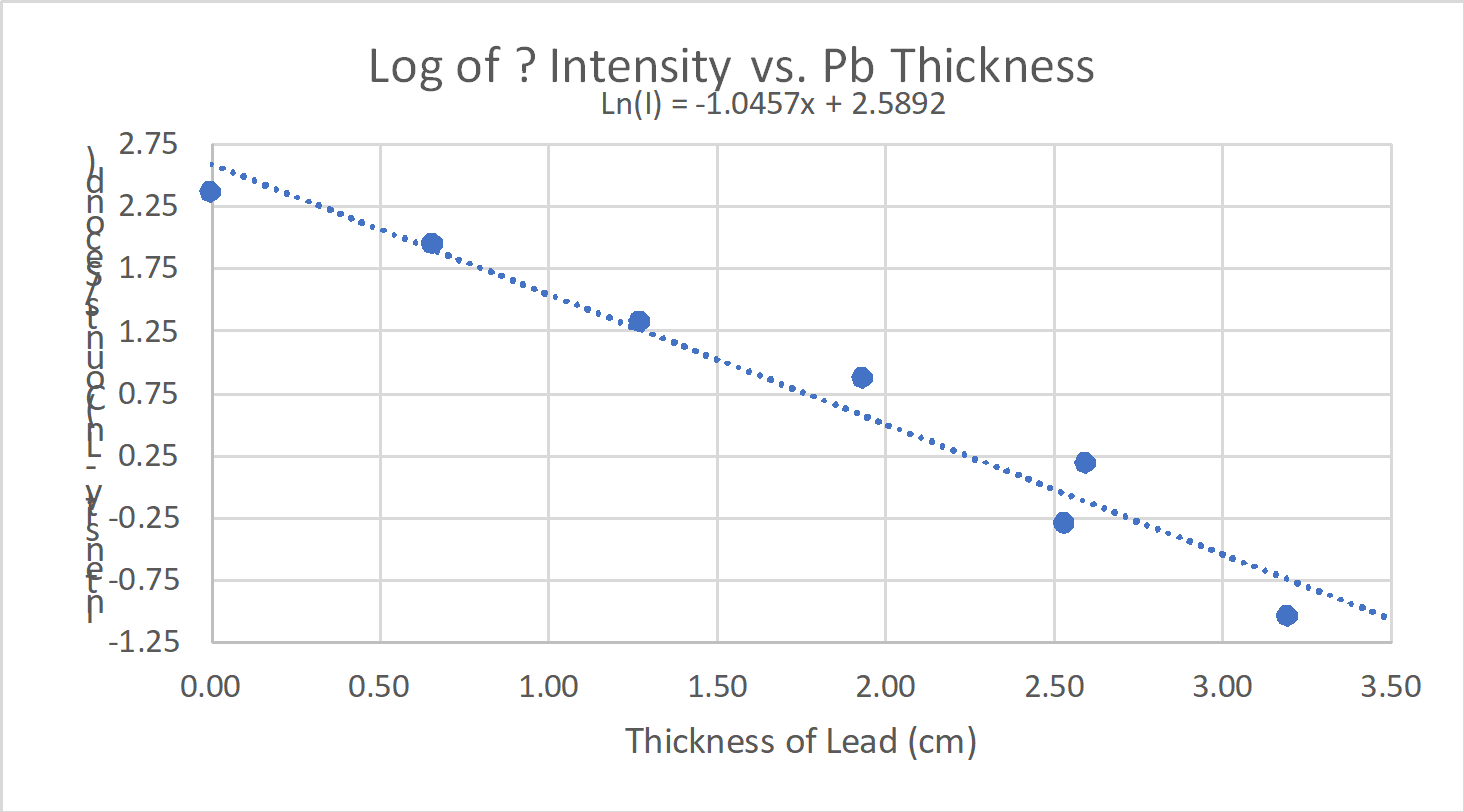
\includegraphics[scale=0.75]{lnivsx} 
  \centering
  \caption{By taking the natural logarithm, we were able to obtain the absorption coefficient $\mu$, equal to 1.0457$cm^{-1}$.}
  \end{figure}
  
  We wanted to compare our result with the literature values provided in the last page of the lab manual. In order to do so, we plotted a graph of photon energy versus absorption coefficient and saw where our experimental value lied within our graph. This qualitative approach is only valid because the gamma rays expelled by the Cesium-137 source used in this experiment are mono-energetic, with a value of $0.662MeV$. The graph is the following:

 \begin{figure}[h]
  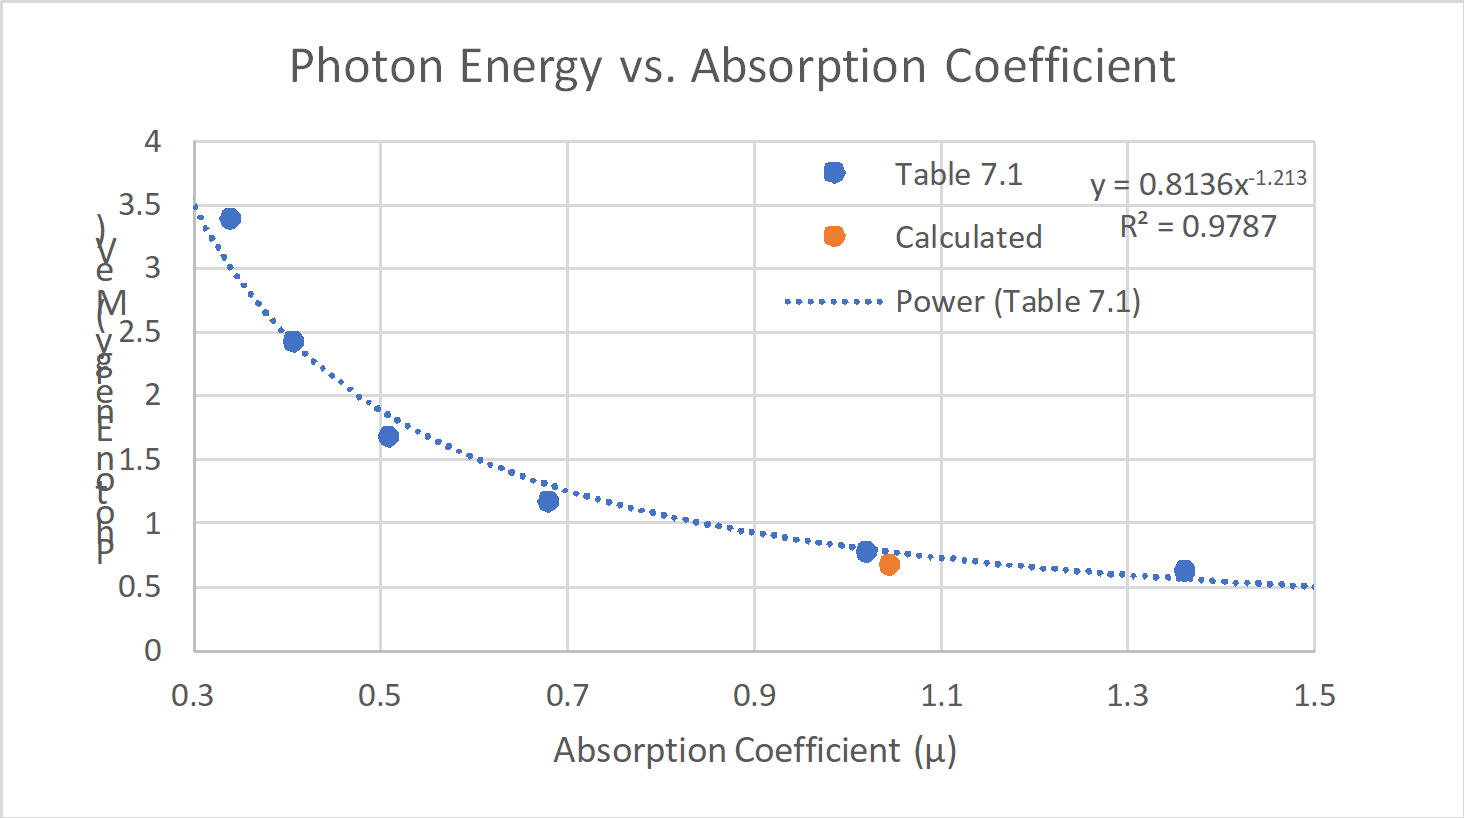
\includegraphics[scale=0.75]{energyvscoeff} 
  \centering
  \end{figure}
  
  As we can see, the photon energy lies very close to the literature value portrayed in the blue line, data extracted form Table 7.1. A future approach to this experiment should consider the possibility of using other energetic gamma rays to verify experimentally this data set.
  
\clearpage
\section{Conclusion}

The results obtained helped us gained a strong qualitative and quantitative understanding of the phenomenon of gamma ray radiation and its detection. The G-M tube was investigated, and its pulses were tweaked and analyzed, and even the intrinsic properties of our apparatus were calculated. We were able to create and examine a real life example where Poisson Distribution occurred, and we even used the recently learned idea of 'chi-squared' goodness of fit. We gained a intuitive understanding of the overwhelmingly complicated oscilloscope, learning to use key aspects such as the CURSOR function, PERSISTENCE mode, scaling, channel variation, etcetera. Overall, this experiment helped us learn a lot about the detection of gamma rays via the G-M tube. Ultimately on the big picture we learned that lead is a very good shield against gamma ray radiation.  We also learned that our hypothesis that an extrinsic resistor would decrease decay time was true.  

At the end of this experiment we were able to complete the goal and obtain the absorption coefficient of lead for a gamma ray of $0.611MeV$. For the future, another experiment that could be done to increase understanding of this phenomenon is the replication of this experiment with gamma rays of different energy. If that was done, the last graph could be checked experimentally and even quantitatively . 

Using a known resistance and capacitor we were able to calculate the intrinsic properties of the counter, with a charge of $4.4nC$,  a capacitance of $7.7nF$ and a resistance of $850\Omega$. 

Using the $\chi^{2}$ goodness of fit, we were able to show that the counting statistics followed the Poisson Distribution to a degree of confidence of 66.4 per cent. 

We were able to calculate the dead time, $\tau=560\mu s$.

We observed that count rate is reduced as lead thickness increases. The measured absorption coefficient for lead under $0.662MeV$ of photon energy is $1.0457cm^{-1}$.
  
\end{document}